The n-channel MOSFET (2N7000) is characterized using the circuit below:

% Circuit diagram

The source and drain are both formed by a metal-semiconductor junction with an n-type region in a p-type substrate. These regions exist in a p-type substrate. The gate is formed by placing an insulating oxide between a metal contact and the aforementioned p-type substrate. When a high voltage is applied at the gate, this attracts attracts excess electrons toward the gate. The electrons cannot leave the substrate due to the insulating oxide layer. So, they simply build up just below the oxide. The number of electrons in this region, known as the channel, increases considerably. However, by the principle of low-level injection ($\delta p$ << $p$ under a perturbation, the applied voltage in this case), the number of holes in the p-type substrate does not change considerably. The conductivity of a semiconductor is given by equation (\ref{eq:cond_semi}):

\begin{equation}
	\label{eq:cond_semi}
	\sigma = q(\mu_n n + \mu_p p)
\end{equation}

Here, $\sigma$ is the conductivity, $q$ is the elementary charge, $\mu_n$ is the electron mobility, $\mu_p$ is the hole mobility, $n$ is the electron concentration, and $p$ is the hole concentration. Since $p$ does not change very much, but $n$ increases considerably, $\sigma$ increases. At a certain point, the channel essentially acts like a conductor. Electrons can now move freely between the source and drain terminals (reference - mosfet_op).

The situation is actually a bit more complicated. Depletion regions exist between the source and the gate and the gate and the drain. When $V_{GS}$ exceeds a threshold voltage, call it $V_{Th}$, the depletion region is overcome, much like in a pn-junction diode. Since the channel acts as a conductor, electrons, the majority carrier in the source, can now flow freely into the channel between the source and drain terminals.

Once the electrons have migrated from the source to the channel, the drain-source voltage, or $V_{DS}$ becomes important. Assume the MOSFET is in the "on" state in which $V_{GS} > V_{Th}$. The channel conductance is essentially constant and given by equation (\ref{eq:cond_semi}). Thus, the channel can be modeled as a simple resistor. By increasing $V_{D}$ and therefore $V_{DS}$, the drain can attract electrons more strongly, causing a greater electron current to flow from the drain. So, for small variations in $V_{DS}$, $I_{D}$ increases approximately linearly with $V_{DS}$.

However, this trend cannot continue indefinitely. At a certain point, electrons are so strongly attracted to the drain, that the channel loses many electrons, causing its conductivity to drop. This causes the drain current $I_{D}$ to taper off since the effect of attracting electrons to the drain by increasing $V_{DS}$ is counteracted by the drop in channel conductance. However, with a sufficiently high $V_{DS}$, the voltage may be high enough to produce a strong enough electric field to force electrons from the source through the channel to the drain.

% Expected plot here

If $V_{DS}$ is held constant and $V_{GS}$ is increased, eventually, $V_{DG}$ drops. If $V_{G}$ becomes sufficiently large relative to $V_{D}$, then the depletion region is not going to be strong enough to actually drive carrier electrons into the drain. So, a larger electron current flows from the channel, but the gate-drain depletion region resists the flow of electrons into the drain. These two effects balance one another out and cause the drain current to level off.

% Describe saturation vs. triode regions.
% Put down expected plots.

The circuit in figure (\ref{fig:mosfet_circ}) is used to plot the MOSFET curves.

\begin{figure}[h!]
\centering
\caption{MOSFET Measurement Circuit}
\label{fig:mosfet_circ}
\begin{circuitikz}
	\draw
	( 0 , 0 ) node[ nmos ] (my_nmos) {}
	(my_nmos.G) to [ R ] ++( -2 , 0 ) coordinate(r_in)
	(my_nmos.G) node[label={ [font=\normalsize] above : $V_{GS}$ } ] { }
	(r_in) to [ battery , v<=$V_1$ ] ++( 0 , -2 ) coordinate(gnd_1)
	(gnd_1) node[ ground ] (my_gnd_1) {}
	(my_nmos.D) node[ ground ] (my_gnd_2) {}
	(my_nmos.S) to [ R , i<_=$I_D$] ++( 0 , 2 ) coordinate(r_c)
	(my_nmos.S) node[label={ [font=\normalsize] below : $V_{DS}$ } ] { }
	(r_c) to [ battery , v<=$V_2$ ] ++( 2 , 0 ) coordinate(gnd_3)
	(gnd_3) node[ ground ] (my_gnd_3) {}
	;
\end{circuitikz}
\end{figure}

To acquire the $I_D$ versus $V_{GS}$ plot, $V_2$ is fixed at $10$\siunitx{\volt}. $V_1$ is varied to observe different measurement points. It should be noted that because the oxide layer prevents current from flowing from the gate's metal contact to the substrate, no current flows through the gate. Thus, the gate voltage $V_G$ is simply $V_1$. Since the source is grounded, $V_S = 0$, which implies that $V_{GS} = V_G - V_S = V_G = V_1$. % Add more details The data in table (\ref{tab:mosfet_id_vds}) below corroborates these claims.

\FloatBarrier

\begin{table}[h!]
	\centering
	\caption{MOSFET $I_D$ versus $V_{GS}$ Data}
	\label{tab:mosfet_id_vgs}
	\csvautotabular{../tables/mosfet_id_vgs.csv}
\end{table}

\FloatBarrier

\FloatBarrier

\begin{figure}[h!]
	\centering
	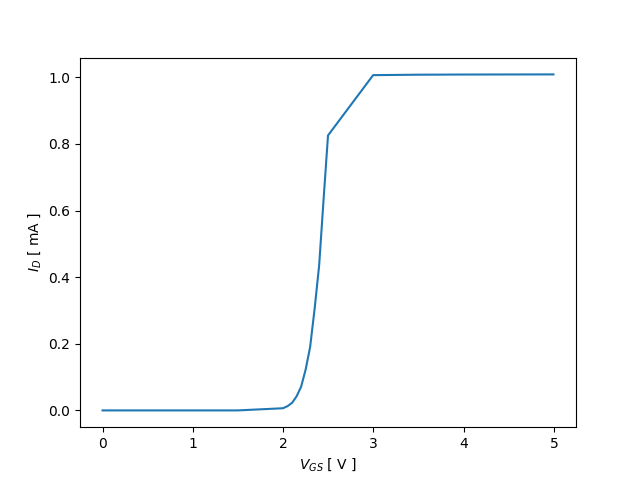
\includegraphics[scale=0.75]{../images/mosfet_id_vgs.PNG}
	\caption{MOSFET $I_D$ versus $V_{GS}$ Plot}
	\label{fig:mosfet_id_vgs}
\end{figure}

\FloatBarrier

The plot in figure (\ref{fig:mosfet_id_vgs}) is precisely as predicted. The MOSFET turns on when $V_{GS}$ exceeds the threshold voltage $V_{Th}$, which is slightly above $2$\siunitx{\volt}. The drain current $I_{D}$ rises exponentially as $V_{GS}$ increases since a larger electron current can now be driven from the channel. Eventually, the curve levels off because the gate voltage $V_{G}$ becomes sufficiently large relative to the drain voltage $V_{D}$, which begins to counteract the flow of electrons into the drain.

To acquire the $I_D$ versus $V_{DS}$ plot, $V_1$ is fixed at about $2.3$\siunitx{\volt}, which is around $V_{Th}$ for the MOSFET as predicted by the previous results. Thus, $V_{GS}$ is fixed. Increasing $V_2$ also increases the drain voltage $V_{D}$ and thus $V_{DS}$ since $V_{DS} = V_D - V_S = V_D$.

\FloatBarrier

\begin{table}[h!]
	\centering
	\caption{MOSFET $I_D$ versus $V_{DS}$ Data}
	\label{tab:mosfet_id_vds}
	\csvautotabular{../tables/mosfet_id_vds.csv}
\end{table}

\FloatBarrier

\FloatBarrier

\begin{figure}[h!]
	\centering
	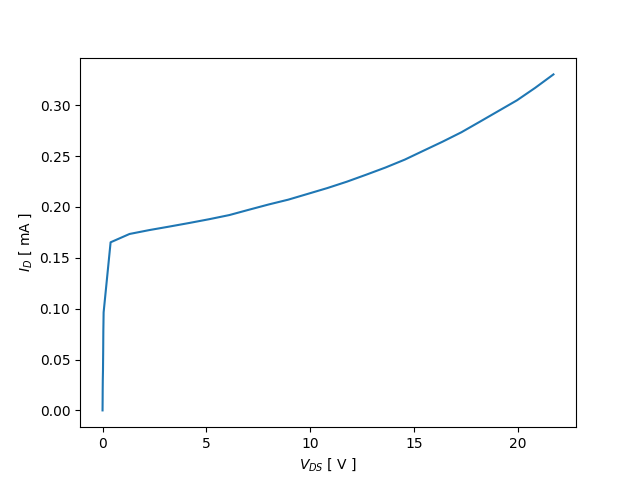
\includegraphics[scale=0.75]{../images/mosfet_id_vds.PNG}
	\caption{MOSFET $I_D$ versus $V_{DS}$ Plot}
	\label{fig:mosfet_id_vds}
\end{figure}

\FloatBarrier

Refs
https://coefs.uncc.edu/dlsharer/files/2012/04/J3b.pdf - mosfet_op
